% Histogram dan Poligon Frekuensi dengan TikZ
% Dokumen LaTeX utuh, siap dikompilasi (butuh paket tikz).
% Data: 32 nilai ulangan harian Matematika kelas 8C, dikelompokkan
% menjadi 6 interval. 40-49: 2 | 50-59: 4 | 60-69: 7
% 70-79: 9 | 80-89: 7 | 90-100: 3
\documentclass{article}
\usepackage{tikz}

\begin{document}

\section*{Histogram: batang menempel, tanpa celah}

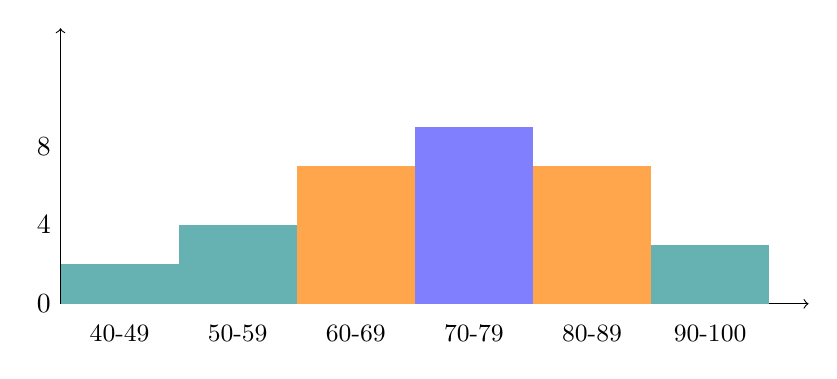
\begin{tikzpicture}
  % sumbu: x = interval nilai, y = frekuensi
  % skala: 1 cm = 4 anak, sumbu frekuensi mulai dari NOL
  \draw[->] (0,0) -- (9.5,0);
  \draw[->] (0,0) -- (0,3.5);
  \foreach \y/\label in {0/0, 1/4, 2/8}
    \node[left] at (0,\y) {\label};
  % batang MENEMPEL: tiap interval lebar 1,5 cm, tinggi = frekuensi / 4
  \fill[teal!60]   (0,0) rectangle (1.5,0.5);   % 40-49: 2
  \fill[teal!60]   (1.5,0) rectangle (3,1);     % 50-59: 4
  \fill[orange!70] (3,0) rectangle (4.5,1.75);  % 60-69: 7
  \fill[blue!50]   (4.5,0) rectangle (6,2.25);  % 70-79: 9
  \fill[orange!70] (6,0) rectangle (7.5,1.75);  % 80-89: 7
  \fill[teal!60]   (7.5,0) rectangle (9,0.75);  % 90-100: 3
  % label interval, tepat di tengah tiap batang
  \foreach \x/\t in {0.75/40-49, 2.25/50-59, 3.75/60-69,
                      5.25/70-79, 6.75/80-89, 8.25/90-100}
    \node[below, font=\small] at (\x,-0.15) {\t};
\end{tikzpicture}

\section*{Poligon frekuensi: menghubungkan titik tengah}

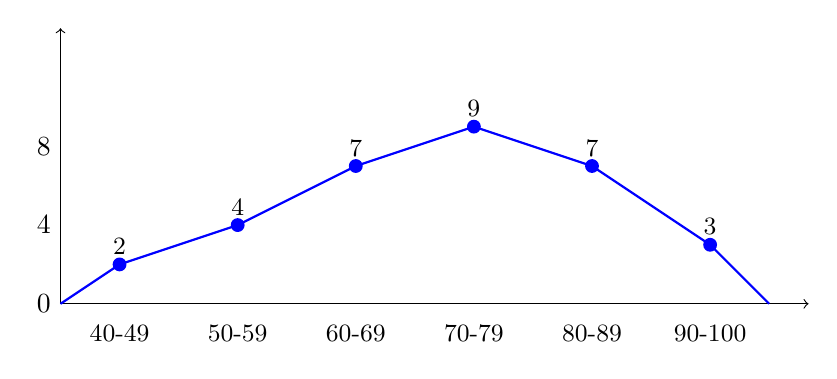
\begin{tikzpicture}
  % sumbu sama seperti histogram di atas
  \draw[->] (0,0) -- (9.5,0);
  \draw[->] (0,0) -- (0,3.5);
  \foreach \y/\label in {0/0, 1/4, 2/8}
    \node[left] at (0,\y) {\label};
  % poligon: mulai (0,0), lewat titik tengah tiap interval, turun ke (9,0)
  \draw[thick, blue] (0,0) -- (0.75,0.5) -- (2.25,1) -- (3.75,1.75)
    -- (5.25,2.25) -- (6.75,1.75) -- (8.25,0.75) -- (9,0);
  \foreach \x/\y/\t in {0.75/0.5/2, 2.25/1/4, 3.75/1.75/7,
                         5.25/2.25/9, 6.75/1.75/7, 8.25/0.75/3}
    { \fill[blue] (\x,\y) circle (2.5pt);
      \node[above, font=\small] at (\x,\y) {\t}; }
  % garis bantu label interval
  \foreach \x/\t in {0.75/40-49, 2.25/50-59, 3.75/60-69,
                      5.25/70-79, 6.75/80-89, 8.25/90-100}
    \node[below, font=\small] at (\x,-0.15) {\t};
\end{tikzpicture}

\end{document}
